\section{Process view}

Ingen af systemets centrale dele gør brug af tråde. Men systemet er opbygget således at afvikling af drone, webapplikation og server kan betragtes som 3 samtidige processer. Alle 3 dele bruges sideløbende i runtime og imellem dem flyder løbende data.

For systemets bruger ser det ud som om al information går direkte fra webapplikation til drone eller omvendt. Men reelt set er webapplikation og drone aldrig i direkte kontakt med hinanden. I stedet går al kommunikation til og fra serveren, som fungerer som et kommunikationslag. 

\vspace{-5pt}
\begin{figure}[H]
	\centering
	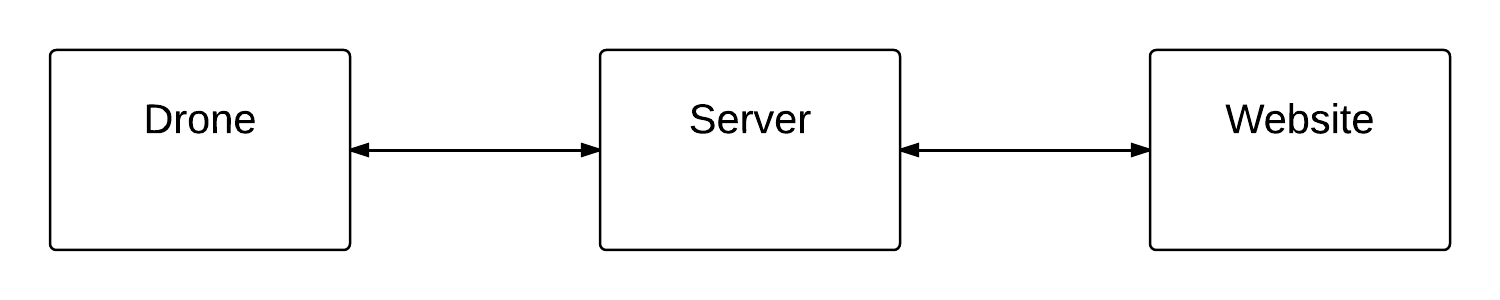
\includegraphics[width=0.7\textwidth]{Billeder/process_view}
	\vspace{0cm}
	\caption{Process view}
	\label{fig:process_view}
\end{figure}

\textbf{Server}\\
Serveren er passiv, hvilket betyder den aldrig tager initiativ til udveksling af data. Serveren foretager ingenting på egen hånd, den står i stedet og venter på at blive igangsat af drone eller webapplikation. 
 
\textbf{Drone} \\
I drone processen håndteres al styring af drone og kommunikation mellem drone og server. Når dronen er tændt og 3G/GPS modulet initialiseret, opdaterer dronen med få minutters interval egen GPS position for efterfølgende at sende serveren information om positionen. Desuden kontrollerer dronen løbende om der er en ny flyveopsætning tilgængelig på serveren. Hvis der er en ny flyveopsætning tilgængelig hentes den, og en ny flyvning påbegyndes. 

\textbf{Webapplikation}\\
Mellem server og webapplikation er der lavet en socket connection. Det betyder at indholdet af webapplikationen opdateres hver gang der kommer nyt indhold på serveren. Desuden bruges webapplikationen når systemets bruger ønsker at lave nye flyveopsætninger eller opdatere de nuværende.\\


Der er lagt megen energi i at designe og bygge systemet på en vis der tillader udvidelser og tilføjelser. Dels kan server nemt tilgås af flere forskellige webapplikationer og desuden kan webapplikationen håndtere flere droner og clienter samtidig.

\newpage
\subsection{Kommunikations timing}
For at kommunikationen mellem drone og server kan fungere optimalt, er der udformet kommunikations timings tabeller. Timings tabellerne foreskrive hvilke request drone skal sende til server og hvilke svar der forventes fra server. \\


Nedenfor forklares kort hvordan drone kommunikerer med webapplikationen i forbindelse med en autonom flyvning.

\begin{enumerate}
	\item Dronen tændes.
	\item Handling i tabel \ref{tab:kom_drone_server_1} udføres og gentages efterfølgende hvert 5. minut.
	\item Handling i tabel \ref{tab:kom_drone_server_2} udføres og gentages hvert 45. sekund indtil der returneres en anden værdi end 0 på NextEvent GET requestet.
	\item Handling i tabel \ref{tab:kom_drone_server_3} udføres
	\item Drone påbegynder flyvning
\end{enumerate} 


\vspace{0.5cm}


\begin{table}[H]
	\centering
		\begin{tabular}{| m {1.5cm} | m {3.5cm} | m {3.5cm} | m {4.7cm} |}
			\hline
			\textbf{Enhed} & \textbf{HTTP Request} & \textbf{Data} & \textbf{Handling} \\ \hline
			Drone & PUT & Online og Location & Opdatere sin position \newline og sætter sig online\\ \hline
			Server & Response & 200 OK & Giver ok svar \\ \hline
		\end{tabular}
	\caption{Kommunikation drone og server - step 1}
	\label{tab:kom_drone_server_1}
\end{table}

\vspace{0.5cm}

\begin{table}[H]
	\centering
		\begin{tabular}{| m {1.5cm} | m {3.5cm} | m {3.5cm} | m {4.7cm} |}
			\hline
			\textbf{Enhed} & \textbf{HTTP Request} & \textbf{Data} & \textbf{Handling} \\ \hline
			Drone & GET & NextEvent & Efterspørg nextevent værdig \\ \hline
			Server & Response & NextEvent & Retunere drone data \newline med nextevent \\ \hline
		\end{tabular}
	\caption{Kommunikation imellem drone og server - step 2}
	\label{tab:kom_drone_server_2}
\end{table}

\vspace{0.5cm}

\begin{table}[H]
	\centering
		\begin{tabular}{| m {1.5cm} | m {3.5cm} | m {3.5cm} | m {4.7cm} |}
			\hline
			\textbf{Enhed} & \textbf{HTTP Request} & \textbf{Data} & \textbf{Handling} \\ \hline
			Drone & GET & Waypoint & Dronen henter waypoints \newline tilhørende event\\ \hline
			Server & Response & Waypoints & Retunere waypoints \newline tilhørende event \\ \hline
			Drone & PUT & NextEvent = 0 & Dronen ændre sin \newline NextEvent værdig til 0 \\ \hline
			Server & Response & 200 OK & Giver ok svar \\ \hline
		\end{tabular}
	\caption{Kommunikation imellem drone og server - step 3}
	\label{tab:kom_drone_server_3}
\end{table}
